\chapter{Zeitplan}
Im folgenden Abschnitt wird der Zeitplan vorgestellt, nach welchem während der IPA 
gearbeitet wurde.

\section{Erläuterung zum Zeitplan}
Der Zeitplan auf der folgenden Seit stellt pro Einheit, eine Stunde dar. Die Balken in den
dunklen Farben repräsentieren die Soll-Stunden, die unteren in den hellen Farben die effektiv-Stunden.
Die drei Sprints welche in dieser IPA durchgeführt werden, sind mit unterschiedlichen Farben gekennzeichnet.

\section{Sprints}
Die IPA wurde in drei unterschiedliche Sprints aufgeteilt: 

\begin{table}[h!]
  \begin{tabular}{|L{0.3\textwidth}|L{0.4\textwidth}|L{0.3\textwidth}|}
      \hline
      \rowcolor{puzzleblue} \color{white}\textbf{Sprint} & \color{white}\textbf{Ziel} & \color{white}\textbf{Datum} \\[12pt]
      \hline
      Initialisierung & Planung und Beschrieb der Arbeit abschliessen & 04.03.2025 \\
     \hline
     Umsetzung & Konzept und Umsetzung selbst abschliessen & 11.03.2025 \\
     \hline
     Finalisierung & Details in der Dokumentation verbessern & 19.01.2025 \\
     \hline
    \end{tabular}
    \caption{Sprintziele}
\end{table}

\newpage

\storeareas\zeitplan
\KOMAoptions{paper=a3, paper=landscape, DIV=current}
\areaset
  {\dimexpr\the\paperwidth-1cm\relax}% calculate requiered \textwidth
  {\dimexpr\the\paperheight-5.5cm\relax}% calculate requiered \textheight
\recalctypearea

\begin{figure}[htp] \centering{
  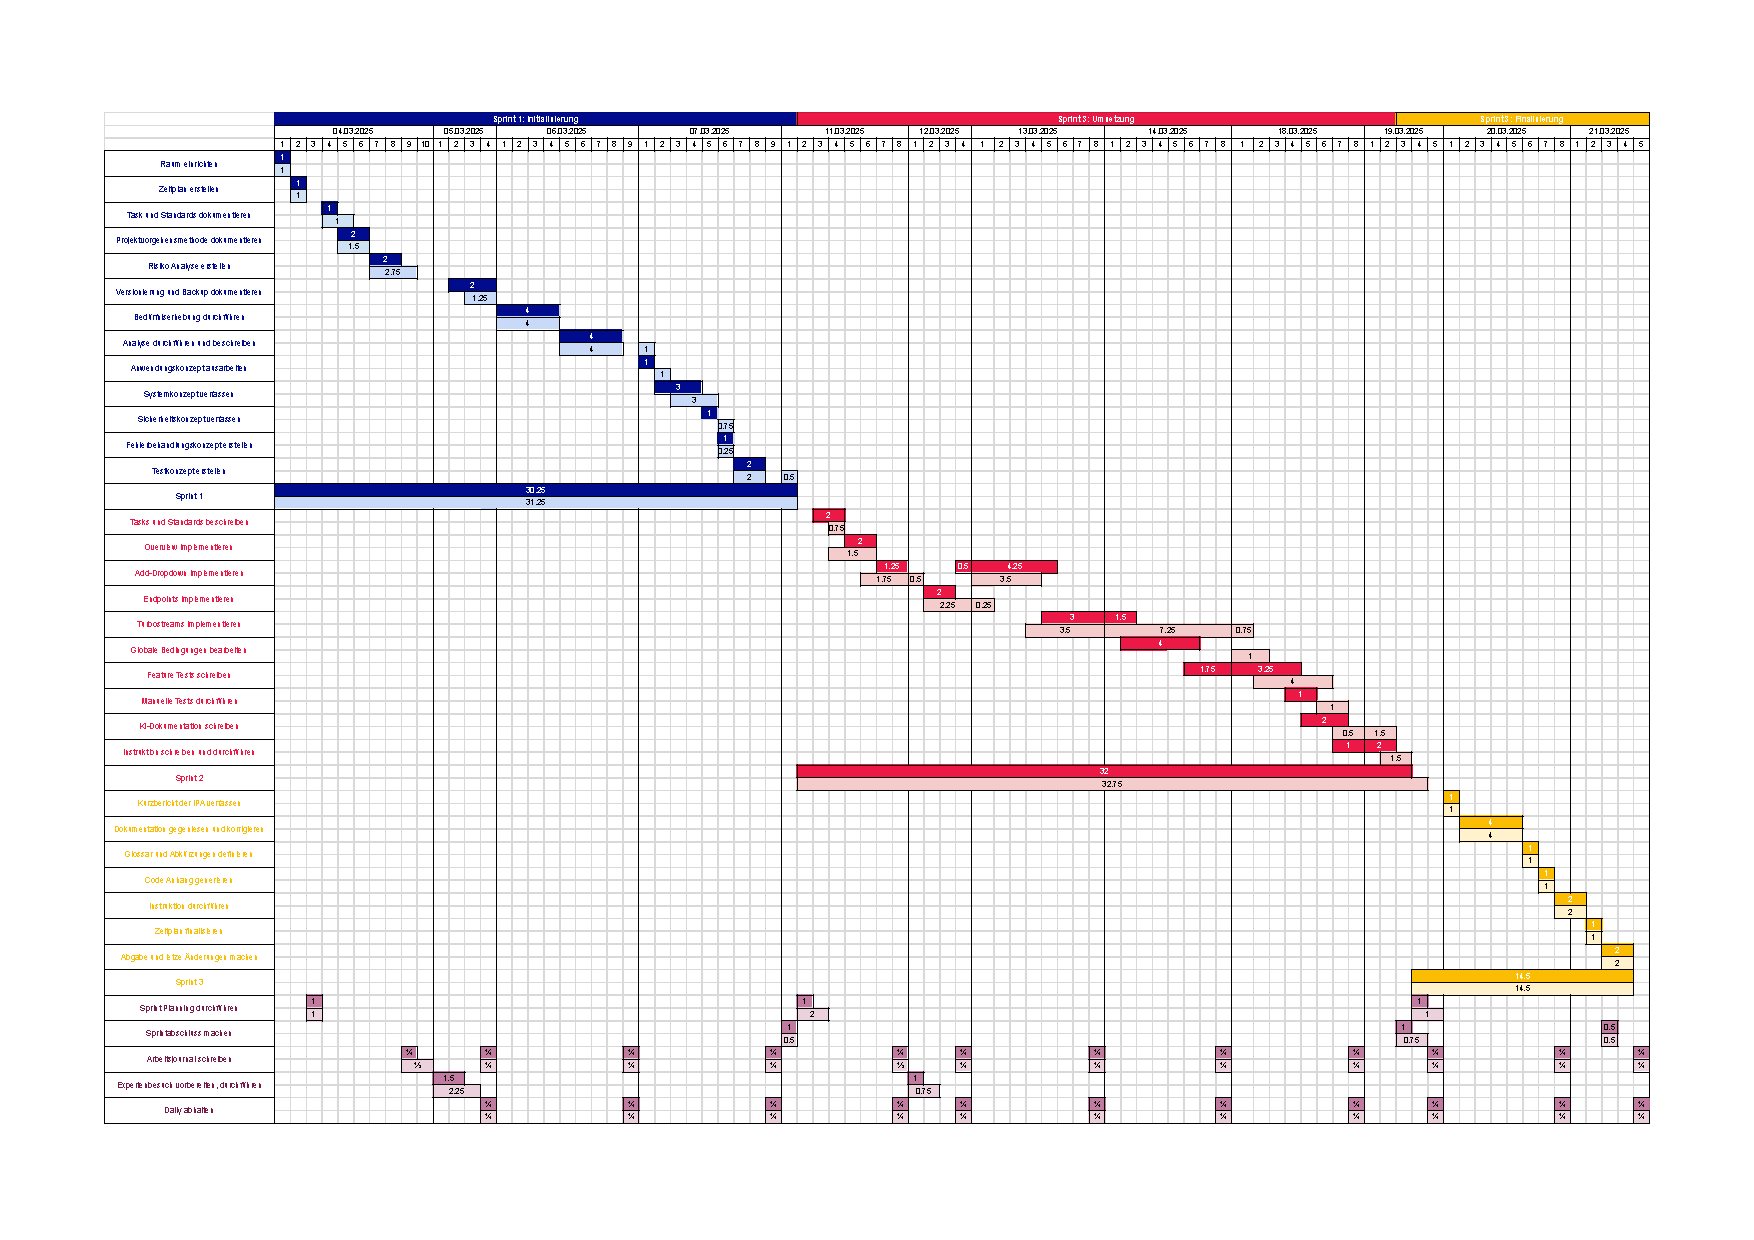
\includegraphics[scale=1.3]{Zeitplan.pdf}}
  \caption{Zeitplan IPA}
\end{figure}

\restoregeometry
\zeitplan
\newpage

